\documentclass{beamer}

\usepackage{hyperref}
\hypersetup{
  pdfinfo={
    CreationDate={D:20180702102722},
    ModDate={D:20180702102722},
  },
}

\AtBeginSection[]
{
  \begin{frame}
    \frametitle{Table of Contents}
    \tableofcontents[currentsection]
  \end{frame}
}

\usetheme{metropolis}
% Some configurations of metropolis theme
\metroset{block=fill}
\metroset{numbering=none}
% Set some custom colors for the beamer theme
\definecolor{DarkBlue}{HTML}{163a7a}
\definecolor{jr@medblue}{RGB}{103,169,207}
\definecolor{jr@green}{RGB}{77,175,74}
\definecolor{jr@darkred}{RGB}{153,0,0}
\setbeamercolor{frametitle}{bg=DarkBlue}
\setbeamercolor{progress bar}{fg=black}
\setbeamercolor{progress bar}{bg=black}
\setbeamercolor{background canvas}{bg=white}
% Use serif font for math
\usefonttheme[onlymath]{serif}
% Margins
\setbeamersize{text margin left=0.5cm,text margin right=0.5cm}
% Slide footer (optional)
\setbeamertemplate{footline}[text line]{%
\parbox{\linewidth}{\vspace*{-0.5cm}\small\hspace{11.15cm}%
\parbox{1cm}{\raggedleft\scriptsize\insertframenumber}}}
\setbeamertemplate{navigation symbols}{}

% lmss uses the computer modern tt font, better for URLs, etc.
\newcommand{\lmss}{\fontfamily{lmtt}\selectfont}

\title[Lagrange and B\'{e}zier]
  {High-order Solution Transfer between Curved Meshes and
  Ill-conditioned B\'{e}zier Curve Intersection}
\date{August 9, 2018}
\author{Danny Hermes}
\institute{{\lmss dhermes@berkeley.edu} \\
           UC Berkeley}
\titlegraphic{
  \vspace{5cm}\hfill
  
\includegraphics[height=1.5cm]{uc_berkeley_seal.pdf}
  \hspace{1.5cm}
}

\begin{document}

\maketitle

%%%%%%%%%%%%%%%%%%%%%%%%%%%%%%%%%%%%%%%%%%%%%%%%%%%%%%%%%%%%%%%%%%%%%%%%%%%%%%%%
%%%   OUTLINE   %%%%%%%%%%%%%%%%%%%%%%%%%%%%%%%%%%%%%%%%%%%%%%%%%%%%%%%%%%%%%%%%
%%%%%%%%%%%%%%%%%%%%%%%%%%%%%%%%%%%%%%%%%%%%%%%%%%%%%%%%%%%%%%%%%%%%%%%%%%%%%%%%
\begin{frame}
\centering
{\Large\bf Outline} \\
\rule{0.82\textwidth}{1pt} \\[20pt]
\begin{minipage}{0.78\textwidth}\raggedright
\begin{enumerate}
\item Introduction and motivation
\item Solution Transfer
\item Compensated Evaluation
\item Modified Newton's for Intersection
\end{enumerate}
\end{minipage}
\end{frame}

%%%%%%%%%%%%%
%%% INTRO %%%
%%%%%%%%%%%%%

\begin{frame}
\centering
{\Large \bf Introduction and motivation}
\rule{0.82\textwidth}{1pt}
\end{frame}

\begin{frame}
\frametitle{A Work in Two Parts: Solution Transfer}
\begin{itemize}
\item Lagrangian Methods
\item Remeshing / rezoning
\item Mesh adaptivity
\item Multiphysics
\item Conservation
\item Curved and / or High-order
\end{itemize}
\end{frame}

\begin{frame}
\frametitle{Method of Characteristics}
To solve the simple transport equation
\begin{equation*}
u_t + c u_x = 0, \quad u(x, 0) = u_0(x).
\end{equation*}
\pause
Divide the physical domain via
\begin{equation*}
x(t) = x_0 + ct
\end{equation*}
\pause
and the PDE becomes a (trivial) ODE
\begin{equation*}
\frac{d}{dt} u(x(t), t) = 0.
\end{equation*}
\end{frame}

\begin{frame}
\frametitle{Method of Characteristics}
\begin{center}
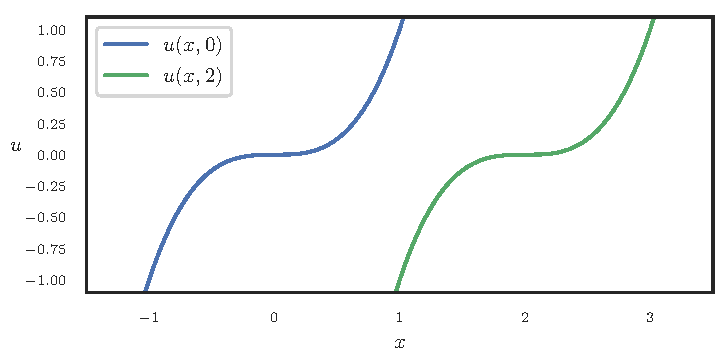
\includegraphics[width=0.95\textwidth]
                {../images/solution-transfer/simple_transport.pdf}
\end{center}
\end{frame}

\begin{frame}
\frametitle{A Work in Two Parts: Ill-conditioned B\'{e}zier}
A
\end{frame}

%%%%%%%%%%%%%
%%% Foo %%%
%%%%%%%%%%%%%

\begin{frame}
\frametitle{Images Needed}
Side-by-side of triangle vs. curved element that is visibly
not convex.
\end{frame}

\begin{frame}
\frametitle{Images Needed}
Side-by-side of triangle intersection vs. curved element intersection
that splits into two parts.
\end{frame}

\end{document}
